\documentclass{beamer}
\usepackage{times}
\usepackage[czech]{babel}
\usepackage[utf8]{inputenc}
\usetheme{Madrid}
\usepackage{graphicx}
\usepackage{amsmath}
\setbeamertemplate{caption}[numbered]
\usepackage{color}

\title{Typografie a publikování -- projekt 5}
\subtitle{Zásobník}
\author{Evgeniya Taipova (xtaipo00)}
\date{\today}
\institute
{
	Vysoké učení technické v~Brně\\
	Fakulta informačních technologií
}

\begin{document}
  \frame{\titlepage}

  \begin{frame}
    \frametitle{Obsah}
    
    \begin{itemize}
      \item Definice
      \item Operace
      \item Příklad použití zásobníku
    \end{itemize}
  \end{frame}

  \begin{frame}
    \frametitle{Definice}
   Je to dynamická datová struktura, umožňující vkládání a odebírání hodnot, přičemž
naposledy vložená hodnota se odebere jako první.
Je to paměť typu LIFO ( zkratka z angl. Last-In First-Out; poslední dovnitř, první ven).
\newline
\begin{center}
 \scalebox{0.2}{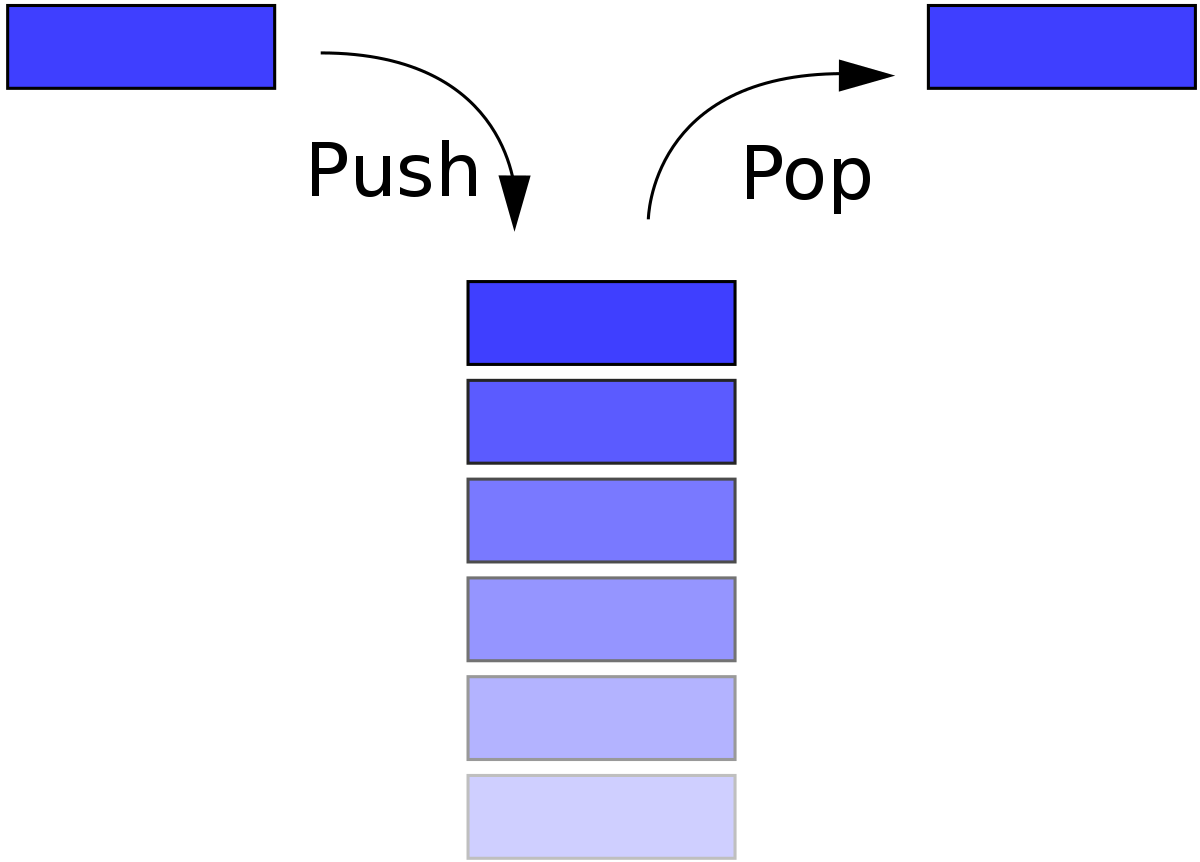
\includegraphics{pp.png}}   
\end{center}
  \end{frame}
  
  \begin{frame}
    \frametitle{Operace}
   Základní operace:
   \begin{itemize}
       \item vložení hodnoty na vrchol zásobníku
       \item odebrání hodnoty z vrcholu zásobníku
       \item test na prázdnost zásobníku
   \end{itemize}
  \end{frame}
 
  \begin{frame}
   Příklad třídy realizující zásobník znaků:
   \begin{center}
      \textcolor{blue}{class} ZasobnikZnaku \{ \newline
\textcolor{blue}{public} ZasobnikZnaku() \{...\}\newline
\textcolor{blue}{public void} vloz(char z) \{ ... \}\newline
\textcolor{blue}{public char} odeber() \{ ... \}\newline
\textcolor{blue}{public boolean} jePrazdny() \{ ... \}\newline
...\newline
\} 
   \end{center}
 Poznámky
\begin{itemize}
\item v angličtině se operace nad zásobníkem obvykle jmenují push, pop a isEmpty
\item pro zásobník může být definována ještě operace čtení hodnoty z vrcholu
zásobníku bez jejího odebrání (v angl. top či peek)
\end{itemize}
 Implementací zásobníku se prozatím nebudeme zabývat, ukážeme si nejprve jeho
použití.
  \end{frame}

 \begin{frame}
    \frametitle{Příklad použití zásobníku}
    Kontrola párování závorek - program, který přečte výraz obsahující tři druhy
závorek a zkontroluje jejich správné párování
\begin{itemize}
\item příklad správného párování: \{ [ ] ( ) \}
\item příklad nesprávného párování: \{ [ ( ] ) \}
\end{itemize}
    \end{frame}
    
  \begin{frame}
      Nástin řešení:
      \begin{enumerate}
          \item  Postupně projdeme všechny znaky tvořící výraz. Pro každý znak mohou nastat tři případy:
          \begin{itemize}
              \item znakem je otevírací závorka: Uložíme ji do zásobníku.
              \item znakem je zavírací závorka: Ze zásobníku (musí být neprázdný)
odebereme naposledy uloženou otevírací závorku a zjistíme, zda
odpovídá zavírací závorce. Pokud neodpovídá, tak nastala chyba
párování.
\item jiný znak: Žádná operace.
          \end{itemize}
\item Po zpracování všech znaků výrazu musí být zásobník prázdný (pokud není, pak
chybí zavírací závorky).
      \end{enumerate}
  \end{frame}
  
  \begin{frame}
    \frametitle{Závěr}
    \begin{center}   
      Děkuju za pozornost
    \end{center}
  \end{frame}
\end{document}
